Целью работы в текущем семестре являлось исследование журнальных файлов и доработка программного модуля для сбора пользовательских данных приложения Google Chrome и представления их в формате XML.

В ходе изучения работы данного браузера было установлено, что приложение Google Chrome хранит пользовательские данные локально. Адреса директорий, используемых по умолчанию для этих целей Google Chrome можно увидеть в таблице~\ref{tab:tab_1}, пользовательские данные --- в таблице~\ref{tab:tab_2}.

\begin{table}[ht]
\caption{Директории хранения журнальных файлов Chrome}
\label{tab:tab_1}
\begin{center}
\begin{tabularx}{\linewidth}{|l|X|}
\hline
Операционная система & Директория \\
\hline
Linux (Debian) & /home/имя пользователя/.config/google-chrome/Default/ \\
\hline
Win7 & C:\textbackslash Users\textbackslash имя пользователя \textbackslash AppData\textbackslash Local\textbackslash Google \\
 & \textbackslash Chrome\textbackslash User Data\textbackslash Default\textbackslash \\
\hline
Win8 & C:\textbackslash Users\textbackslash имя пользователя \textbackslash AppData\textbackslash Local\textbackslash Google \\
 & \textbackslash Chrome\textbackslash User Data\textbackslash Default\textbackslash \\
\hline
\end{tabularx}
\end{center}
\end{table}

\begin{table}[ht]
\caption{Пользовательские данные}
\label{tab:tab_2}
\begin{center}
\begin{tabularx}{\linewidth}{|l|X|}
\hline
Файл & Содержание \\
\hline
Bookmarks & Закладки \\
\hline
History & История посещений, история запросов, история загруженных файлов \\
\hline
Preferences & Настройки (директория загрузки файлов, версия программы, логин аккаунта Google) \\
\hline
Login Data & Сохраненные логины и пароли \\
\hline
Extensions (папка) & Расширения \\
\hline
\end{tabularx}
\end{center}
\end{table}

\subsubsection{База данных Login Data Chrome}

Login Data --- это реляционная база данных, основанная на СУБД SQLite.
Необходимо рассмотреть данную БД, которая содержит 2 таблицы:

\begin{enumerate}
  \item logins;
  \item meta.
\end{enumerate}

Интерес представляет только таблица logins. Она содержит следующие поля:

\begin{enumerate}
  \item origin\_url --- адрес ресурса;
  \item username\_value --- логин для доступа;
  \item password\_value --- пароль, представленный в виде BLOB массива двоичных данных (Binary Large OBject);
  \item date\_created --- дата сохранения, представленная в следующем виде (пример): 13072972925957814. Это число есть количество секунд, прошедшее с 00:00:00 UTC 1 января, 1601 года (рис.~\ref{ship_1:ship_1}).
\end{enumerate}

\begin{figure}[h!]
\center{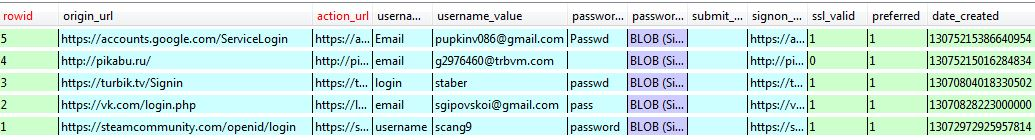
\includegraphics[width=0.9\linewidth]{ship_1}}
\caption{Структура таблицы login}
\label{ship_1:ship_1}
\end{figure} 

Запрос для импорта данных выглядит следующим образом:

\begin{verbatim}
SELECT logins.origin_url,
       logins.username_value,
       datetime(logins.date_created/1000000 + 
       (strftime('%s','1601-01-01')),'unixepoch')
FROM logins;
\end{verbatim}

Результат выполнения запроса можно увидеть на рисунке~\ref{ship_2:ship_2}, блок-схему алгоритма выборки данных из БД Login Data --- на рисунке~\ref{ship_3:ship_3}. Результат выполнения программы в формате XML --- рисунок~\ref{ship_4:ship_4}.

Значение поля id --- уникальный идентификатор для последующего импорта в solr БД и работы с ним.

\begin{figure}[h!]
\center{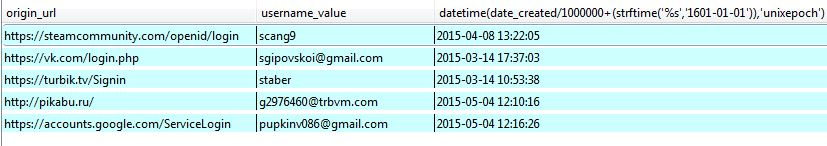
\includegraphics[width=0.9\linewidth]{ship_2}}
\caption{Результат выполнения запроса}
\label{ship_2:ship_2}
\end{figure}

\begin{figure}[h!]
\center{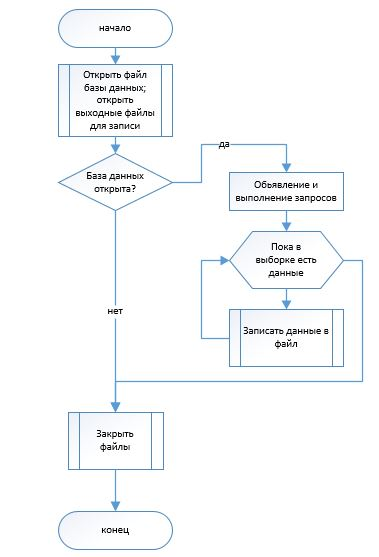
\includegraphics[width=0.5\linewidth]{ship_3}}
\caption{Блок-схема алгоритма выборки данных из БД Login Data}
\label{ship_3:ship_3}
\end{figure} 

\begin{figure}[h!]
\center{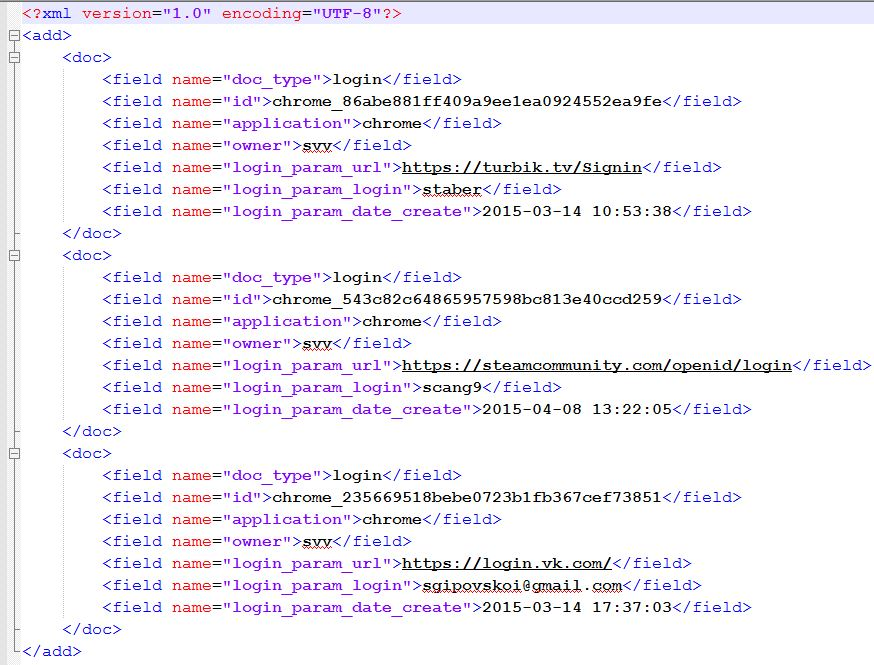
\includegraphics[width=0.7\linewidth]{ship_4}}
\caption{Файл login.XML}
\label{ship_4:ship_4}
\end{figure} 

\clearpage
\subsubsection{Расширения браузера Chrome (Extensions)}

В папке Extensions (рис.~\ref{ship_5:ship_5}) находятся данные об установленных в брузере расширениях. Для каждого расширения имеется своя папка, в которой находится различная информация. Также для каждого Extension имеется файл manifest (рис.~\ref{ship_6:ship_6}) с расширением JSON. JSON (JavaScript Object Notation) --- текстовый формат обмена данными, основанный на JavaScript. Из данного файла необходима только информация об имени и версии расширения.

Блок-схему алгоритма импорта данных о расширениях можно увидеть на рисунке~\ref{ship_7:ship_7}. 

\begin{figure}[h!]
\center{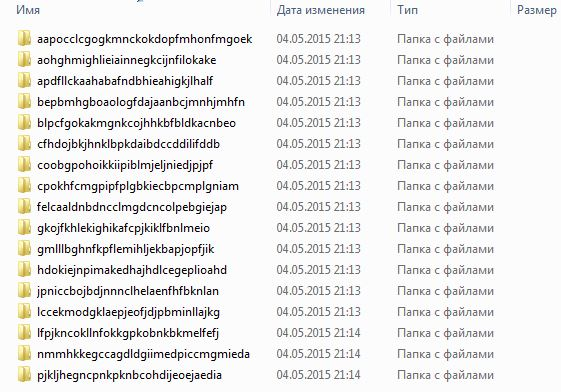
\includegraphics[width=0.6\linewidth]{ship_5}}
\caption{Папка Extensions}
\label{ship_5:ship_5}
\end{figure}

\begin{figure}[h!]
\center{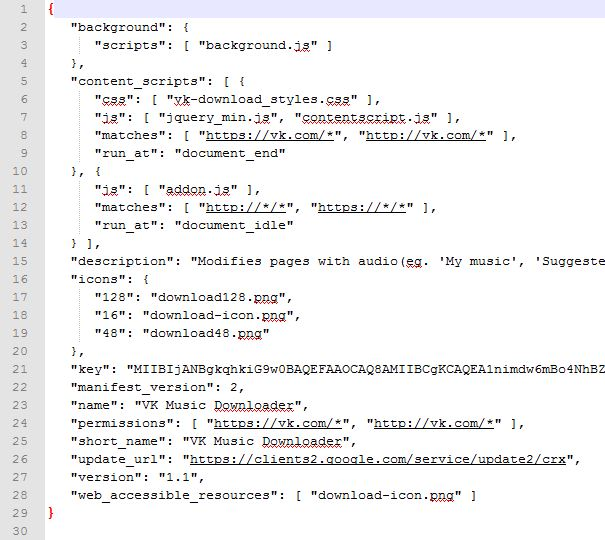
\includegraphics[width=0.6\linewidth]{ship_6}}
\caption{Файл manifest.json}
\label{ship_6:ship_6}
\end{figure}

\begin{figure}[h!]
\center{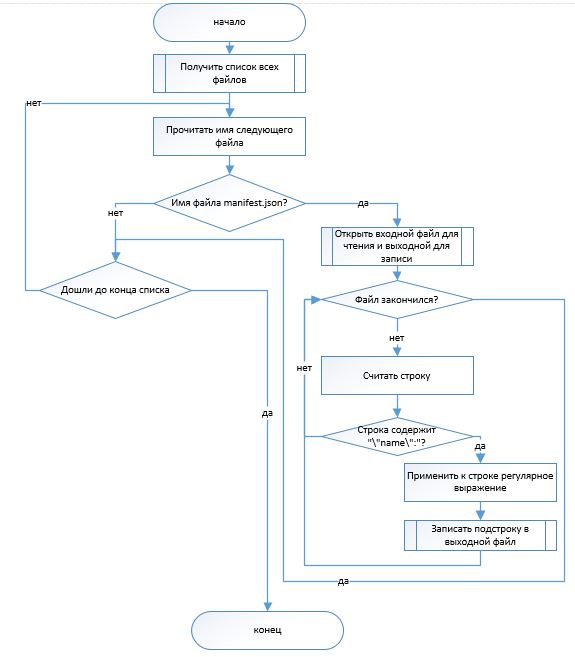
\includegraphics[width=0.8\linewidth]{ship_7}}
\caption{Блок-схема алгоритма импорта данных о расширениях}
\label{ship_7:ship_7}
\end{figure}

\clearpage
Извлечение подстроки из строки осуществляется с помощью регулярного выражения \textbackslash"(.*)\textbackslash".*\textbackslash"(.*)\textbackslash". Например, есть строка <<name>>: <<VK Music Downloader>>. Данное регулярное выражение возвращает 2 подстроки --- <<name>> и <<VK Music Downloader>>, что и требовалось в ходе работы.

Результат был записан в файл extensions.XML (рис.~\ref{ship_8:ship_8}).

\begin{figure}[h!]
\center{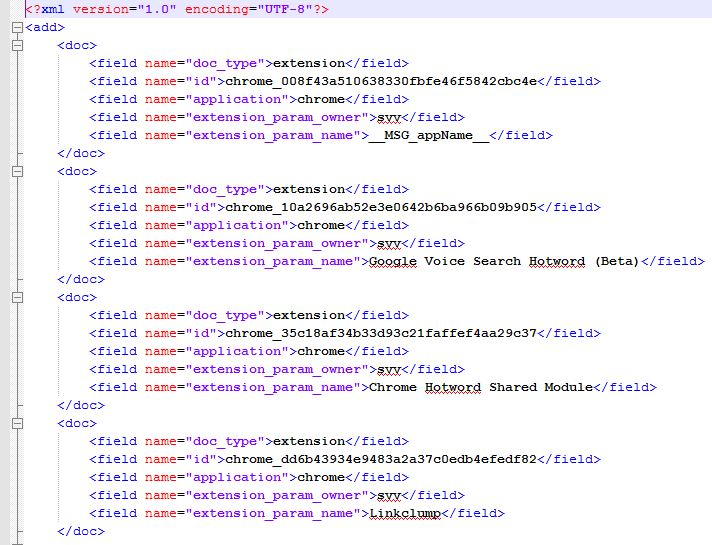
\includegraphics[width=0.7\linewidth]{ship_8}}
\caption{Файл extensions.XML}
\label{ship_8:ship_8}
\end{figure}

\subsubsection{Изменения, добавленные в программный модуль в течение текущего семестра}

В файл bookmarks.XML добавлены 2 поля (рис.~\ref{ship_9:ship_9}):

\begin{enumerate}
  \item дата добавления закладки;
  \item владелец файла.
\end{enumerate}

\begin{figure}[h!]
\center{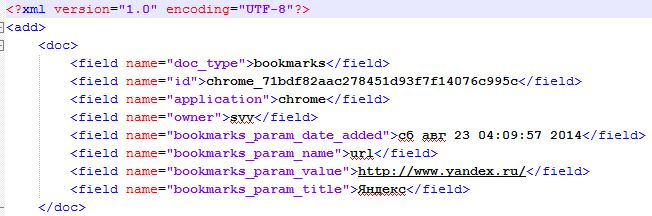
\includegraphics[width=0.7\linewidth]{ship_9}}
\caption{Файл bookmarks.XML}
\label{ship_9:ship_9}
\end{figure}

В файл history.XML (рис.~\ref{ship_10:ship_10}) добавлено поле-дата последнего посещения ресурса.

\begin{figure}[h!]
\center{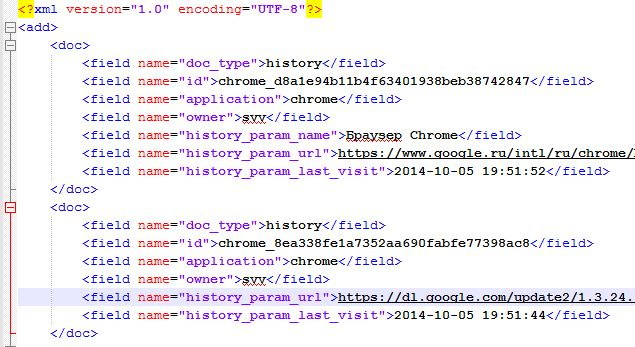
\includegraphics[width=0.8\linewidth]{ship_10}}
\caption{Файл history.XML}
\label{ship_10:ship_10}
\end{figure}

Также было реализовано преобразование данных времени начала и конца загрузки, а также о количестве занимаемого места к читаемому виду (рис.~\ref{ship_11:ship_11}).

\begin{figure}[h!]
\center{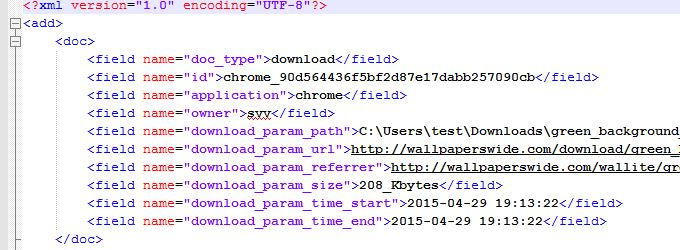
\includegraphics[width=0.8\linewidth]{ship_11}}
\caption{Файл downloads.XML}
\label{ship_11:ship_11}
\end{figure}

\clearpage
Помимо этого реализованы следующие задачи:

\begin{enumerate}
  \item присоединение модуля к общей системе coex;
  \item рекурсивный обход файловой системы для нахождения входных файлов;
  \item различие выходных данных при обработке входных от нескольких пользователей путём добавления в конец имени файла даты и количества наносекунд, прошедших с начала работы функции.
\end{enumerate}

На данный момент реализован импорт следующих данных:

\begin{enumerate}
  \item история посещений;
  \item история загруженных файлов;
  \item история поисковых запросов;
  \item список установленных расширений;
  \item информация о версии программы, подключённом аккаунте google;
  \item сохраненные данные для доступа к ресурсам(только логин).
\end{enumerate}

Список всех выходных XML-файлов приведен на рисунке~\ref{ship_12:ship_12}.

\begin{figure}[h!]
\center{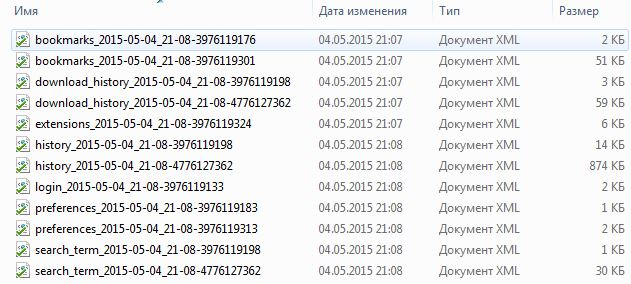
\includegraphics[width=0.7\linewidth]{ship_12}}
\caption{Файл downloads.XML}
\label{ship_12:ship_12}
\end{figure}
